% 学習結果説明（手順3d：学習データの確認。5data 版と Alldata 版。用語集と図の見方）
% results フォルダで「lualatex 学習結果説明_手順3d.tex」を2回実行すると PDF を作り直せる（TeX Live の LuaLaTeX を使用）。
% 図は results/step3d/ の PNG を相対パスで読み込む。
\documentclass[paper=a4paper,fontsize=10.5pt,line_length=44zw,number_of_lines=38]{jlreq}
\usepackage[haranoaji]{luatexja-preset}
\usepackage{amsmath}
\usepackage{graphicx}
\usepackage{booktabs}
\usepackage{tabularx}
\usepackage{enumitem}
\usepackage{float}
\usepackage{xcolor}
\usepackage[hidelinks,bookmarksnumbered]{hyperref}
\graphicspath{{step3d/}}

\newcommand{\file}[1]{\texttt{\detokenize{#1}}}
\newcommand{\gd}{\dot{\gamma}}
\newcommand{\Tff}{T_{\mathrm{ff}}}
\newcommand{\Tset}{T_{\mathrm{set}}}
\newcommand{\PI}{P3\_1}
\newcommand{\PII}{P3\_2}
\newenvironment{termlist}{\begin{itemize}[label=・,leftmargin=1\zw,labelwidth=1\zw,labelsep=0pt,itemsep=0.4ex,topsep=0.6ex,parsep=0pt]}{\end{itemize}}
\newcommand{\term}[1]{\item \textbf{#1}：}
\newenvironment{points}{\begin{itemize}[label=$\triangleright$,leftmargin=1.5\zw,itemsep=0.3ex,topsep=0.5ex,parsep=0pt]}{\end{itemize}}
\newcommand{\pt}[1]{\item \textbf{#1}：}
\renewcommand{\arraystretch}{1.25}

\title{樹脂粘度モデル開発　手順3dの学習結果の説明\\[0.6ex]{\large 学習データの確認（5data 版と Alldata 版）：用語集とグラフの見方（機械学習・統計を初めて学ぶ人向け）}}
\author{}
\date{2026年10月14日}

\begin{document}
\maketitle
{\small\tableofcontents}

% =====================================================================
\section{この文書について}

この文書は、\file{results/step3d/} にある手順3dの結果（図と表）を、機械学習や統計を初めて学ぶ人でも読めるように説明したものです。手順3d は、\textbf{今後の検討（手順5 以降）で使う学習データを、決めて、確かめる}手順です。

\begin{points}
\pt{対象の結果}\file{results/step3d/}：図 5 枚、CSV 8 個。図は、すべて \file{results/step3d/highres/} にも、600 dpi で保存されます（ほかに、せん断速度 ― 粘度のグラフ 28 枚）。
\pt{読み方}2章で何をしたかをつかみ、分からない言葉は3章の用語集で調べてください。4章で図の見方、5章で表の見方、6章で結果のまとめを説明します。
\pt{数値について}文中の数値は、この文書を作った時点の results の表から取り出したものです。
\pt{元のノート}\file{01_機械学習コードフォルダ} の \file{手順3d_学習データの確認.ipynb} です。ノートの先頭に使い方があり、「設定エリア」だけを直せば設定を変えられます。たとえば、\file{DATA\_VERSIONS} で、どちらの版を検討するかを選べます。実行は約 8 分です。
\pt{記号表}記号・モデル名（R3 など）・データの呼び名（5data 版、Alldata 版など）・列名の一覧は、\file{学習結果説明_記号表.pdf} にあります。
\pt{作り直し方}\file{results} フォルダで \texttt{lualatex 学習結果説明\_手順3d.tex} を2回実行すると、この PDF を作り直せます。
\end{points}

% =====================================================================
\section{何をしたか（概要）}

\subsection{目的：学習データを、2 つの版にそろえる}
これまでの手順（3a〜5a）では、目的ごとに、いろいろなファイルを使ってきました（5data、3data、Alldata、no1.5-3.0 など。それぞれに「外れ値あり」と「外れ値なし」）。これでは、結果を比べにくいので、\textbf{今後は、外れ値なしの 2 つの「版」だけを使う}ことにしました（ユーザー決定、2026 年 10 月 14 日）。「版」は、「どのデータで学習して、どのデータで確かめるか」の組み方です。

\begin{table}[H]
\caption{今後使う 2 つの版（どちらも外れ値なしで、問題データ一覧の「除外」を除く）}
\begin{tabularx}{\linewidth}{@{}l>{\raggedright\arraybackslash}p{9\zw}>{\raggedright\arraybackslash}X@{}}
\toprule
版 & 学習 & 確かめ方（検証） \\
\midrule
5data 版 & 5data（93 条件。4〜5 ショット/条件） & 3data で、学習していない速度（低速側 3・5 mm/s、高速側 280・320 mm/s）を予測できるかを確かめる（\textbf{外挿}）。そのほか、5data の 190・230 ℃ で学習して 210 ℃ を予測（S\_T）、5data の中の交差検証（CV）。 \\
Alldata 版 & Alldata（全条件。PP は 1 条件 8〜10 ショット、粉砕材混合 PP は 1〜5 ショット） & 条件単位の 10 分割の交差検証（CV）。S\_T（190・230 ℃ で学習して 210 ℃ を予測。テストは 5data 版と同じ行）。S\_Vall（Alldata のうち 5data の条件だけで学習して、3data を予測）。 \\
\bottomrule
\end{tabularx}
\end{table}

ノートの設定 \file{DATA\_VERSIONS} で、片方だけ、または両方を検討できます。手順5 の本実装は、この 2 つの版に当てはめて、比べます。

\subsection{確かめたこと}
\begin{enumerate}[itemsep=0.4ex,topsep=0.5ex]
\item \textbf{版の中身}：行数・条件数・分け方（表\ref{tab:versions}）。
\item \textbf{ファイルの包含関係}：5data と 3data は、Alldata の一部のはずです。実際に、同じ行かを確かめました（表\ref{tab:incl}）。
\item \textbf{ショットの順番によるずれ}：Alldata は、同じ条件を 10 回（PP）測っています。回を重ねるうちに、金型や樹脂の状態が変わって、粘度が少しずつずれていないかを確かめました（図1、表\ref{tab:drift}）。もしずれていたら、「Alldata の後半のショットを、5data の前半と同じに扱ってよいか」が怪しくなります。
\item \textbf{外れ値の検知}：新しい規則（\textbf{規則 f}）で、「ほかの条件から予測した値と、大きく違う条件」を探しました。拾った外れ値は、問題データ一覧に記録して除いてよい、とユーザーが指示したので（10 月 14 日）、その手順に従いました（図2・図3、表\ref{tab:outlier}）。
\item \textbf{同じモデルでの精度の比較}：基本のモデル R3 で、2 つの版の精度を比べました（図4・図5、表\ref{tab:rmse}〜\ref{tab:nlpd}）。
\end{enumerate}

\subsection{規則 f（外れ値の検知）のしくみ}
\begin{enumerate}[itemsep=0.4ex,topsep=0.5ex]
\item 条件ごとに、ショットの $\ln\eta$ と $\ln\gd$ を平均して、「条件平均」を作ります（PP は 125 点、粉砕材混合 PP は 129 点）。
\item 条件平均から、GPR（入力は条件平均の $\ln\gd$、$\ln H$、$\Tset$。R3 と同じ形）を作ります。ただし、\textbf{条件を 1 つずつ抜いて}、抜いた条件を残りで予測します（これを、全条件で繰り返します）。
\item 実測と予測の差（\textbf{残差}、$\ln\eta$ の単位）を、予測の不確かさ（予測標準偏差）で割った値を \textbf{$z$} とします。$z$ は、「予測の不確かさの何倍、外れているか」です。
\item $|z|>3.5$ \textbf{かつ} |残差| $>0.1$（粘度で約 10\%）のとき、その条件を「候補」として拾います。$z$ だけだと、予測がとても正確な所では、わずかな違いでも拾ってしまうので、残差の大きさ（実用上の違い）も条件にしています。
\item 一覧の「除外」を除いた後のデータでも、もう一度調べます（除いた条件の影に、別の外れ値が隠れていないかを見るため）。
\end{enumerate}
規則 a〜e（手順3 までの候補）は、「見直しの候補」で、外れ値と判定するかはユーザーが決めます。規則 f は、外れ値として、一覧に「除外」で記録してよい規則です（拾った条件が 4 つ以上のときは、登録の前に相談します）。

\subsection{R3 での比較のしくみ}
\begin{table}[H]
\caption{分け方（R3：条件平均の $\gd$、$H$、$\Tset$ の GPR。ARD Matern 5/2 ＋ 線形カーネル ＋ ノイズ）}
\begin{tabularx}{\linewidth}{@{}l>{\raggedright\arraybackslash}p{9\zw}>{\raggedright\arraybackslash}X@{}}
\toprule
分け方 & 5data 版 & Alldata 版 \\
\midrule
S\_V & 5data で学習 $\to$ 3data（外挿）。低速側と高速側に分けて評価 & --- \\
S\_Vall & --- & Alldata のうち 5data の条件（全ショット）で学習 $\to$ 3data。PP は、同じ 93 条件のショットが増えたとき、外挿が良くなるかを見る（粉砕材混合 PP は、5data と同じデータなので、S\_V と同じ） \\
S\_T、S\_T3 & 5data の 190・230 ℃ で学習 $\to$ 5data の 210 ℃（S\_T）、3data の 210 ℃（S\_T3） & Alldata の 190・230 ℃ で学習 $\to$ \textbf{同じ}テスト行（5data ファイルの 210 ℃、3data ファイルの 210 ℃）。そのまま比べられる \\
CV & 5data の中の、条件単位の 10 分割 & Alldata の、条件単位の 10 分割（同じ条件のショットは、同じ側に入れる） \\
\bottomrule
\end{tabularx}
\end{table}

\textbf{注意}：Alldata 版の利点（両端の条件も学習に入る）は、同じデータの中の交差検証（CV）では測れません。CV で、両端の条件を抜いたときの成績は、残りの条件が両端の近くにあるので、5data 版の外挿より、楽になります。5data 版の外挿の成績が、「両端を学習に入れない場合」の目安です。

% =====================================================================
\section{用語集}

\subsection{データの版と、分け方に関する用語}
\begin{termlist}
\term{5data 版・Alldata 版}学習と検証の、データの組み方（2 章の表）。ファイル名の 5data・Alldata は、ファイルそのものの名前で、「版」は、そのファイルを使った学習と検証の組み方です。
\term{外挿・内挿}学習した範囲の外側（外挿）、内側（内挿）の予測。外挿は、一般に、内挿より難しい。
\term{最終モデル（ALL）}その版で、すべての学習データを使って作るモデル。5data 版は 5data、Alldata 版は Alldata の全条件。
\term{交差検証（CV）}データを K 個に分け、1 個ずつを検証、残りを学習にして、K 回繰り返す方法。ここでは、K = 10 で、\textbf{同じ条件のショットが、同じ側に入る}ようにして（条件単位の分割）、学習と検証に同じ条件が入らないようにしました。K 回の予測を集めて、指標を出します。
\term{S\_V、S\_Vall、S\_T、S\_T3}分け方の名前（2 章の表）。\textbf{S\_V}：5data で学習して 3data を予測。\textbf{S\_Vall}：Alldata のうち 5data の条件で学習して 3data を予測。\textbf{S\_T}：190・230 ℃ で学習して、5data の 210 ℃ を予測。\textbf{S\_T3}：同じ学習で、3data の 210 ℃ を予測。
\term{低速側・高速側・内側}射出速度による区分。低速側：3・5 mm/s、高速側：280・320 mm/s、内側：その間。
\term{包含関係}あるファイルの全行が、別のファイルにも入っているか、という関係。ここでは、5data・3data が Alldata の一部か。
\term{問題データ一覧、除外・感度確認}一覧は、問題のある条件を 1 行ずつ記録する表（\file{02_機械学習データ/問題データ一覧.csv}）。\textbf{除外}：解析から除く。\textbf{感度確認}：解析に残し、除いた場合の結果を並べる。手順3dでは、\textbf{P03 を「感度確認」から「除外」に変えました}。
\end{termlist}

\subsection{ショットの順番と、ずれに関する用語}
\begin{termlist}
\term{ショットと、順番（\file{pos}）}同じ条件での、1 回の成形がショット。元ファイル名の先頭の 3 桁は、設定温度・厚みごとの通し番号（速度の条件ごとに連続した番号）なので、条件の中での順番は、\textbf{\file{pos}}（最初のショット = 1）で表します。
\term{条件平均からの偏差}あるショットの値から、その条件の平均を引いた値。条件ごとの違い（粘度の大きさそのもの）を除いて、同じ条件の中のずれだけを見られます。
\term{傾き（1 ショットあたりのずれ）}偏差を、順番 \file{pos} に対して回帰した直線の傾き。正なら、順番が進むと値が増え、負なら減る。「ずれ（最初 $\to$ 最後）」は、傾きに、順番の幅（PP は 9、粉砕材混合 PP は 4）を掛けたもの。
\term{標準誤差}推定した値（傾きなど）が、どれだけ不確かかの目安。傾きが標準誤差の 2 倍より大きければ、偶然ではなさそう、という目安にします。ただし、データが多いと、ごく小さなずれでも、有意になります。大切なのは、ずれの大きさが、実用上の許容値（0.02）より小さいか、です。
\term{純粋誤差}同じ条件のショット間のばらつき（$\ln\eta$ の標準偏差）。手順3a・3b の用語集と同じ。R3 のノイズの標準偏差と比べます。
\end{termlist}

\subsection{外れ値の検知に関する用語}
\begin{termlist}
\term{残差}実測の値から、予測の値を引いた差。ここでは $\ln\eta$ の差で、0.1 は粘度で約 10\% の違い。
\term{$z$（ゼット）}残差を、予測標準偏差で割った値。「予測の不確かさの何倍、外れているか」を表します。目安として、絶対値が 3.5 を超えると、まれな外れ方です。外れ値なしのファイルを作ったときの「修正 $z$ スコア」（Tff に使う）とは、別の指標です。
\term{予測標準偏差}予測の不確かさ。手順3a・3b の用語集と同じ。
\term{条件を 1 つずつ抜く予測}その条件を学習から除いて、残りの条件で予測すること。その条件が、ほかと整合しているかを調べられます。
\term{規則 f}上の 2.3 節のしくみ。$|z|>3.5$ かつ |残差| $>0.1$ の条件を拾います。
\end{termlist}

\subsection{評価に関する用語}
\begin{termlist}
\term{RMSE・被覆率・NLPD}手順3a・3b の用語集と同じです。RMSE は予測の平均的な誤差（$\ln\eta$）、被覆率は 95\% 予測区間に実測が入った割合（0.95 に近いほど、区間の広さが適切）、NLPD は当たり具合と区間の適切さをまとめた指標（小さいほど良い）です。
\term{R3}条件平均の $\gd$、$H$、$\Tset$ を入力にした GPR。CLAUDE.md §6 の比較用の GPR（R1）と同じ形。手順3b で決めた基本のモデルです。
\term{ノイズの標準偏差}GPR が、「ショットごとのばらつき」として学習した値。純粋誤差に近ければ、成形条件から見たばらつきを表しています。
\term{高解像度の保存}ノートの設定 \file{HR\_ALL} が True のとき、すべての図を、600 dpi でも \file{highres/} に保存します（報告書や発表資料に使うため）。
\end{termlist}

% =====================================================================
\section{図の見方}

図ごとに、「何を示す図か」「軸と記号」「見るポイント」「今回の結果」の順に説明します。図のファイルは \file{results/step3d/} にあります。

% ---------------------------------------------------------------------
\subsection{図1：ショットの順番によるずれ（\file{fig1\_shot\_drift.png}）}
\begin{figure}[H]
\centering
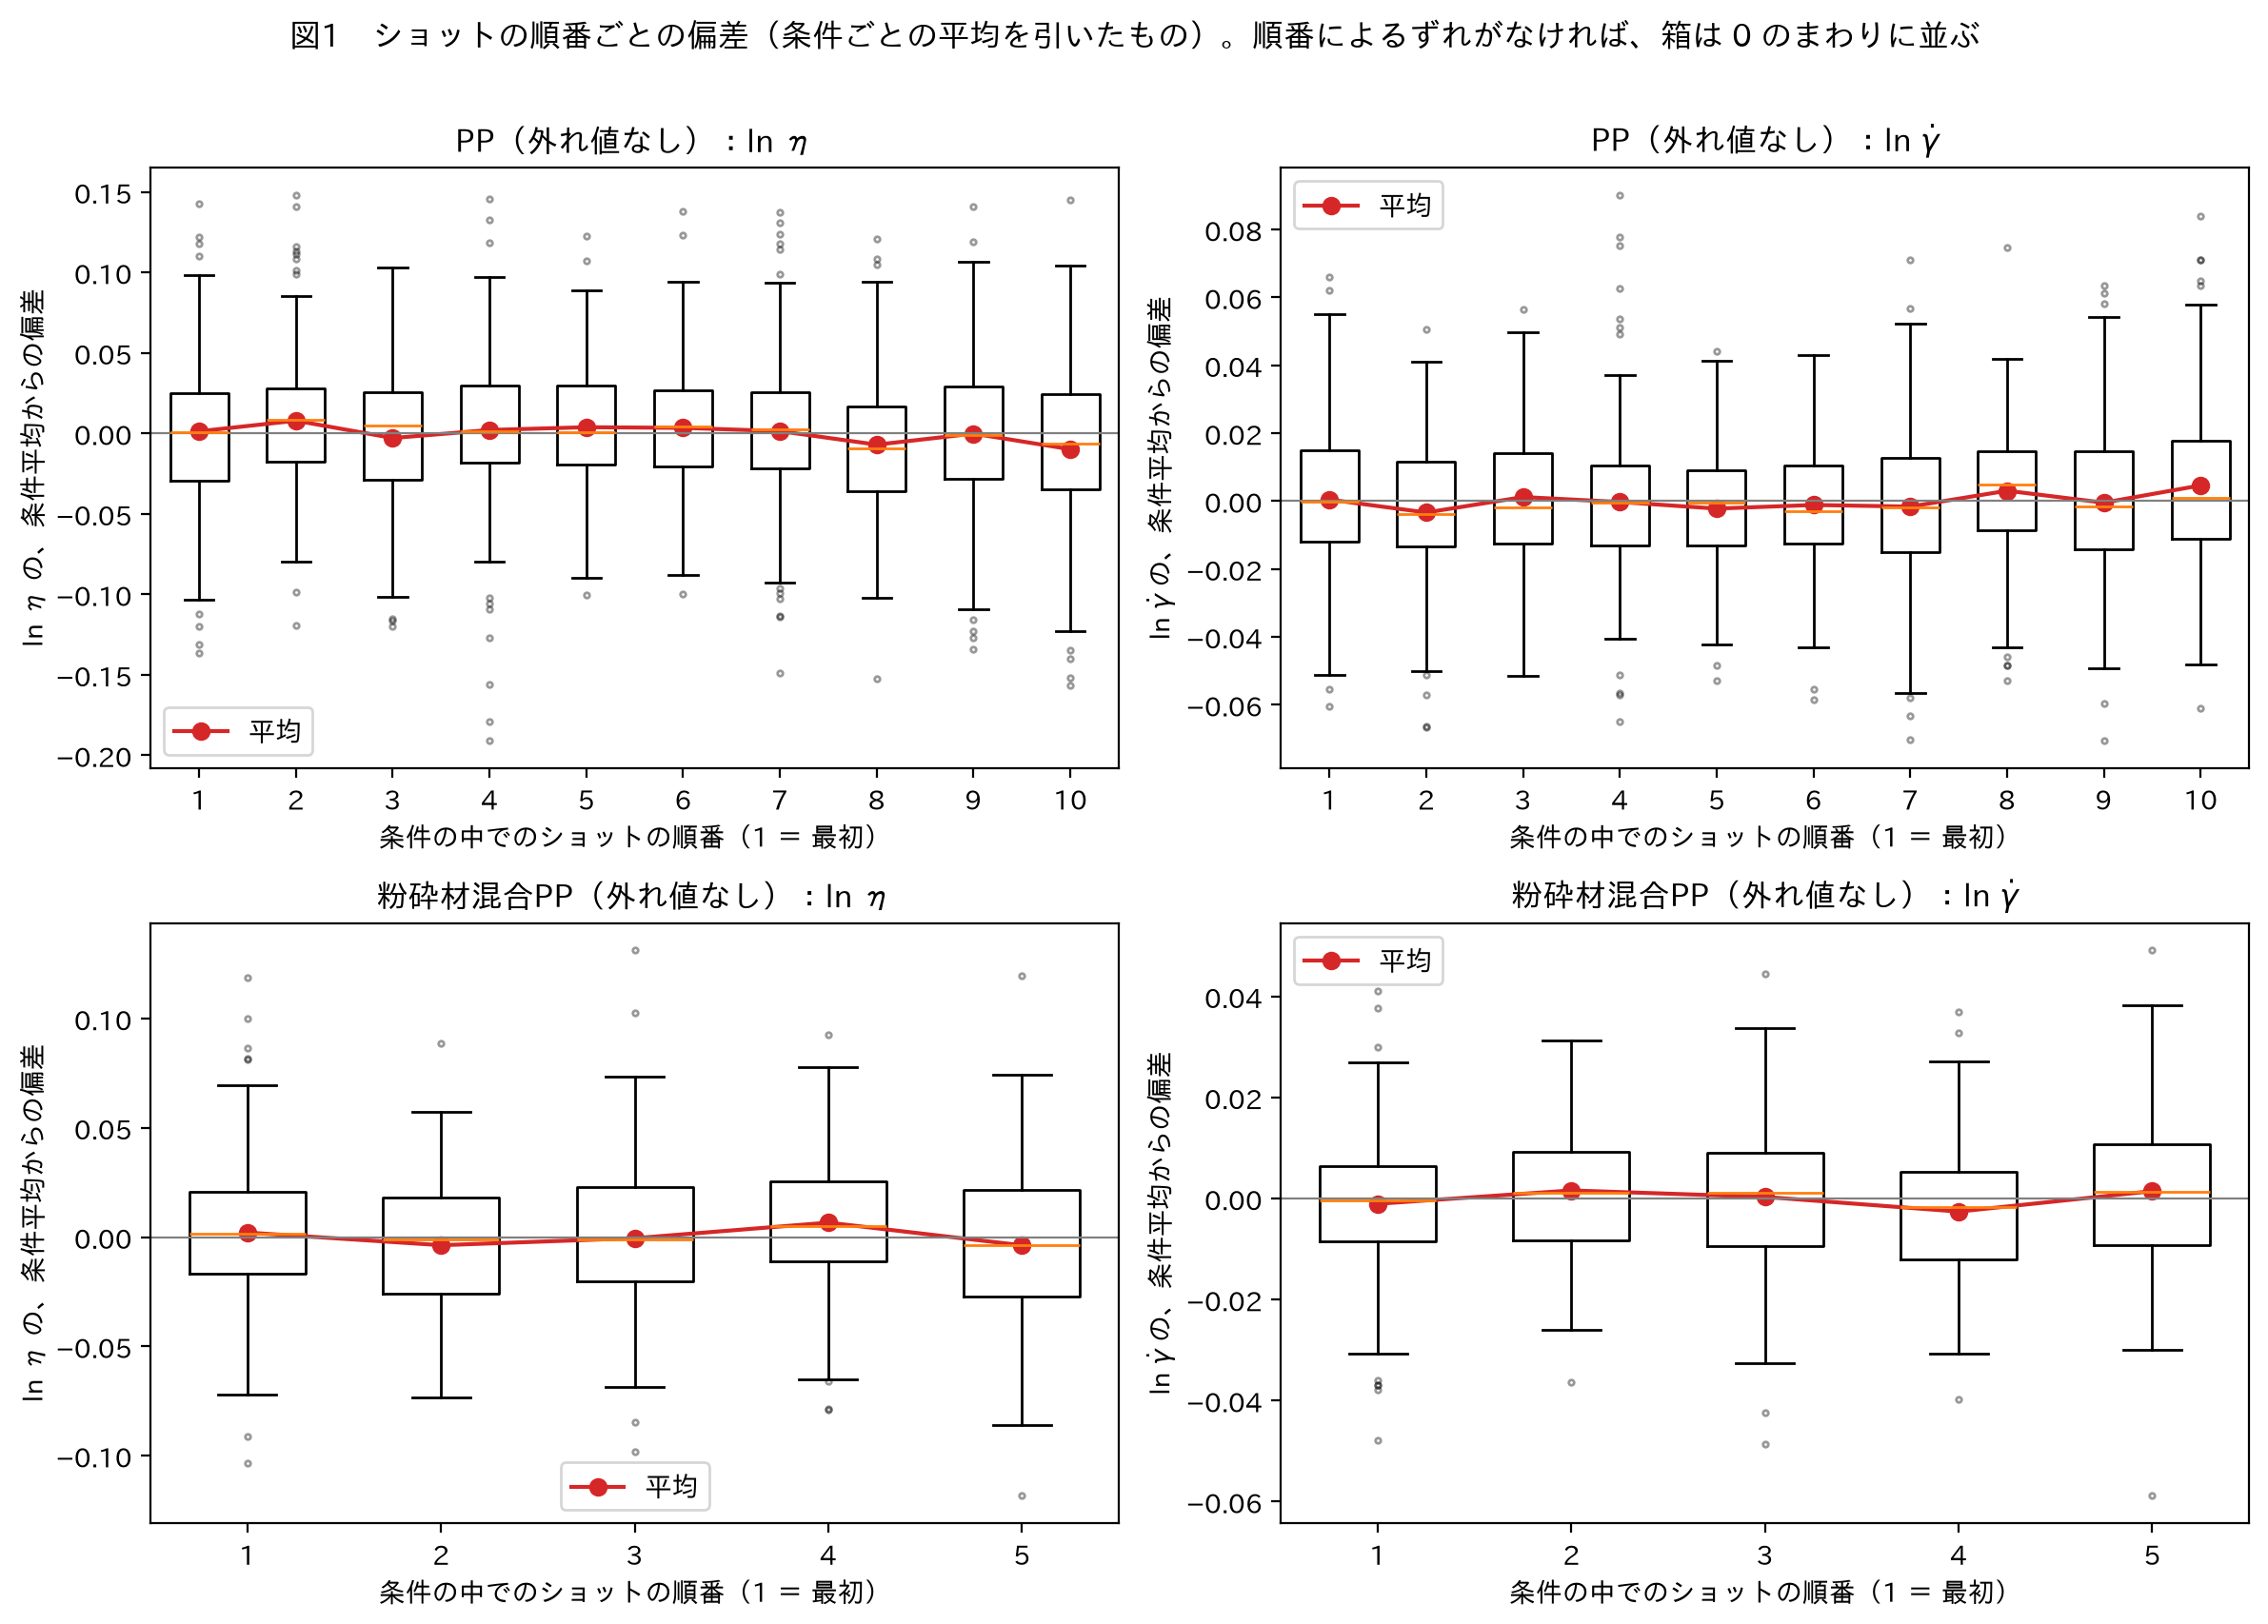
\includegraphics[width=0.95\linewidth]{fig1_shot_drift.png}
\caption{Alldata（外れ値なし）の、ショットの順番ごとの偏差。左が $\ln\eta$、右が $\ln\gd$。上が PP、下が粉砕材混合 PP}
\end{figure}
\begin{points}
\pt{ファイル}\file{results/step3d/fig1_shot_drift.png}（\file{highres/} に 600 dpi 版）。
\pt{何を示す図か}同じ条件の中で、ショットの順番が進むと、値が変わっていくか（ずれ）を見る図です。
\pt{軸と記号}横軸は、条件の中でのショットの順番（1 が最初）。縦軸は、条件の平均を引いた値（偏差）。箱は、順番ごとの、全条件の偏差の分布（箱が中央 50\%、ひげが範囲、小さい点が外れた値）。赤い線は、順番ごとの平均。
\pt{見るポイント}箱が、どの順番でも 0 のまわりに並び、赤い線が右上がり・右下がりでなければ、ずれはありません。
\pt{今回の結果}PP の ln η の箱は、順番 1〜10 のどこでも 0 のまわりにあり、赤い平均の線にも、右上がり・右下がりの傾向は見えません（傾き $-0.00109$ /ショット。標準誤差 0.00051 の約 2.2 倍で、ごくわずかな右下がり。9 ショット分で粘度の約 1.0\%）。粉砕材混合 PP も同じです（順番は 1〜5）。ln $\gd$ の箱も 0 のまわりで、ショットが進んでも、せん断速度は変わっていません。群ごとに見ても、最大は PP の 射出速度 低速側（3・5 mm/s） の $-0.0416$（粘度で約 4\%）で、許容値の 2 倍（0.04）をわずかに超えますが、傾きは標準誤差の約 1.8 倍で、偶然の範囲です（9 条件しかなく、標準誤差が大きいため。「順番 6 以降 $-$ 5 以前」は $-0.0207$）。
\end{points}

% ---------------------------------------------------------------------
\subsection{図2：規則 f の結果（\file{fig2\_outlier\_scan.png}）}
\begin{figure}[H]
\centering
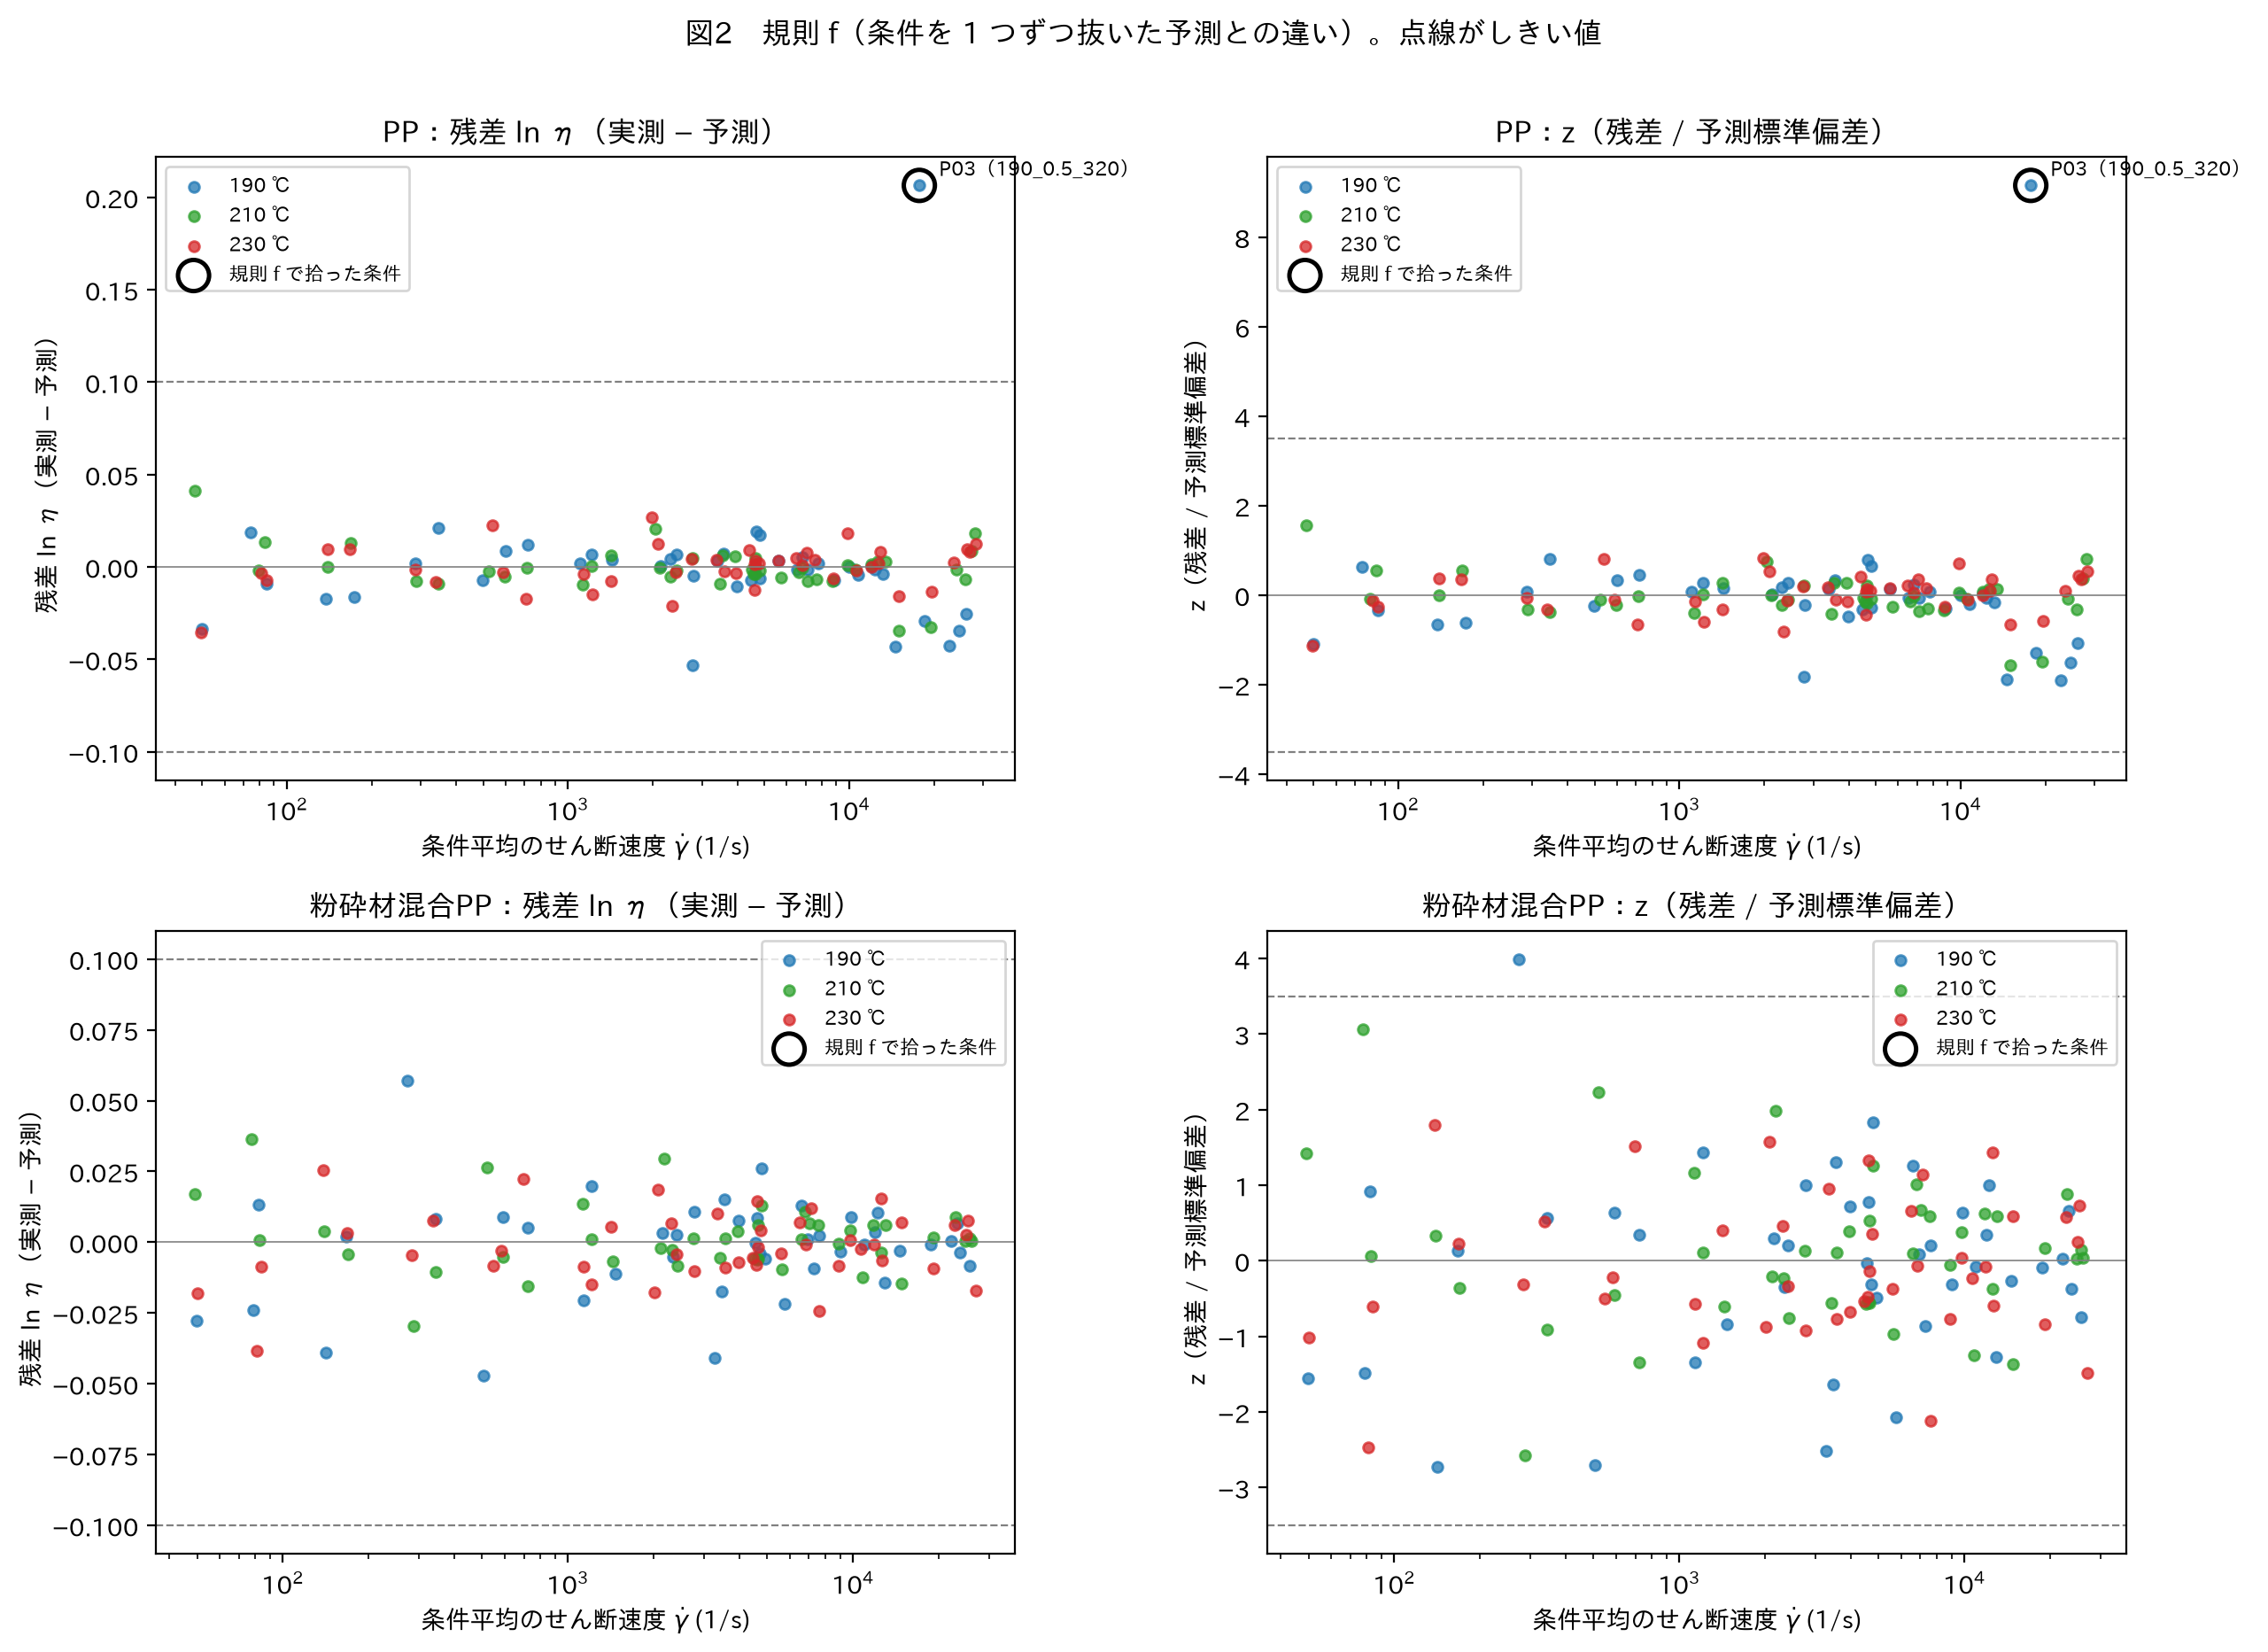
\includegraphics[width=0.95\linewidth]{fig2_outlier_scan.png}
\caption{規則 f：条件ごとの残差（左）と $z$（右）。黒い丸が、拾った条件}
\end{figure}
\begin{points}
\pt{ファイル}\file{results/step3d/fig2_outlier_scan.png}
\pt{何を示す図か}条件を 1 つずつ抜いて予測したとき、実測がどれだけ外れたか、を条件ごとに見る図です（除外する前の全条件）。上が PP、下が粉砕材混合 PP。
\pt{軸と記号}横軸は、条件平均のせん断速度（対数軸）。縦軸は、左が残差（$\ln\eta$）、右が $z$。色は設定温度（青 190 ℃、緑 210 ℃、赤 230 ℃）。点線がしきい値（残差 $\pm$0.1、$z$ $\pm$3.5）。黒い丸が、規則 f で拾った条件で、横に、問題データ一覧の ID と条件名を付けています。
\pt{見るポイント}点が、点線の中に入っているか。外にある点が、拾われる条件です。
\pt{今回の結果}PP の図の右上の 1 点（P03：190 ℃・0.5 mm・320 mm/s）だけが、しきい値（点線）の外にあります（残差 $+$0.21、z = 9.2。粘度は予測の 1.23 倍）。ほかの条件は、残差が $\pm$0.06 以内、z も $\pm$4 以内に収まっています。粉砕材混合 PP は、拾った条件がありません。
\end{points}

% ---------------------------------------------------------------------
\subsection{図3：問題の条件の、全ショット（\file{fig3\_problem\_conditions.png}）}
\begin{figure}[H]
\centering
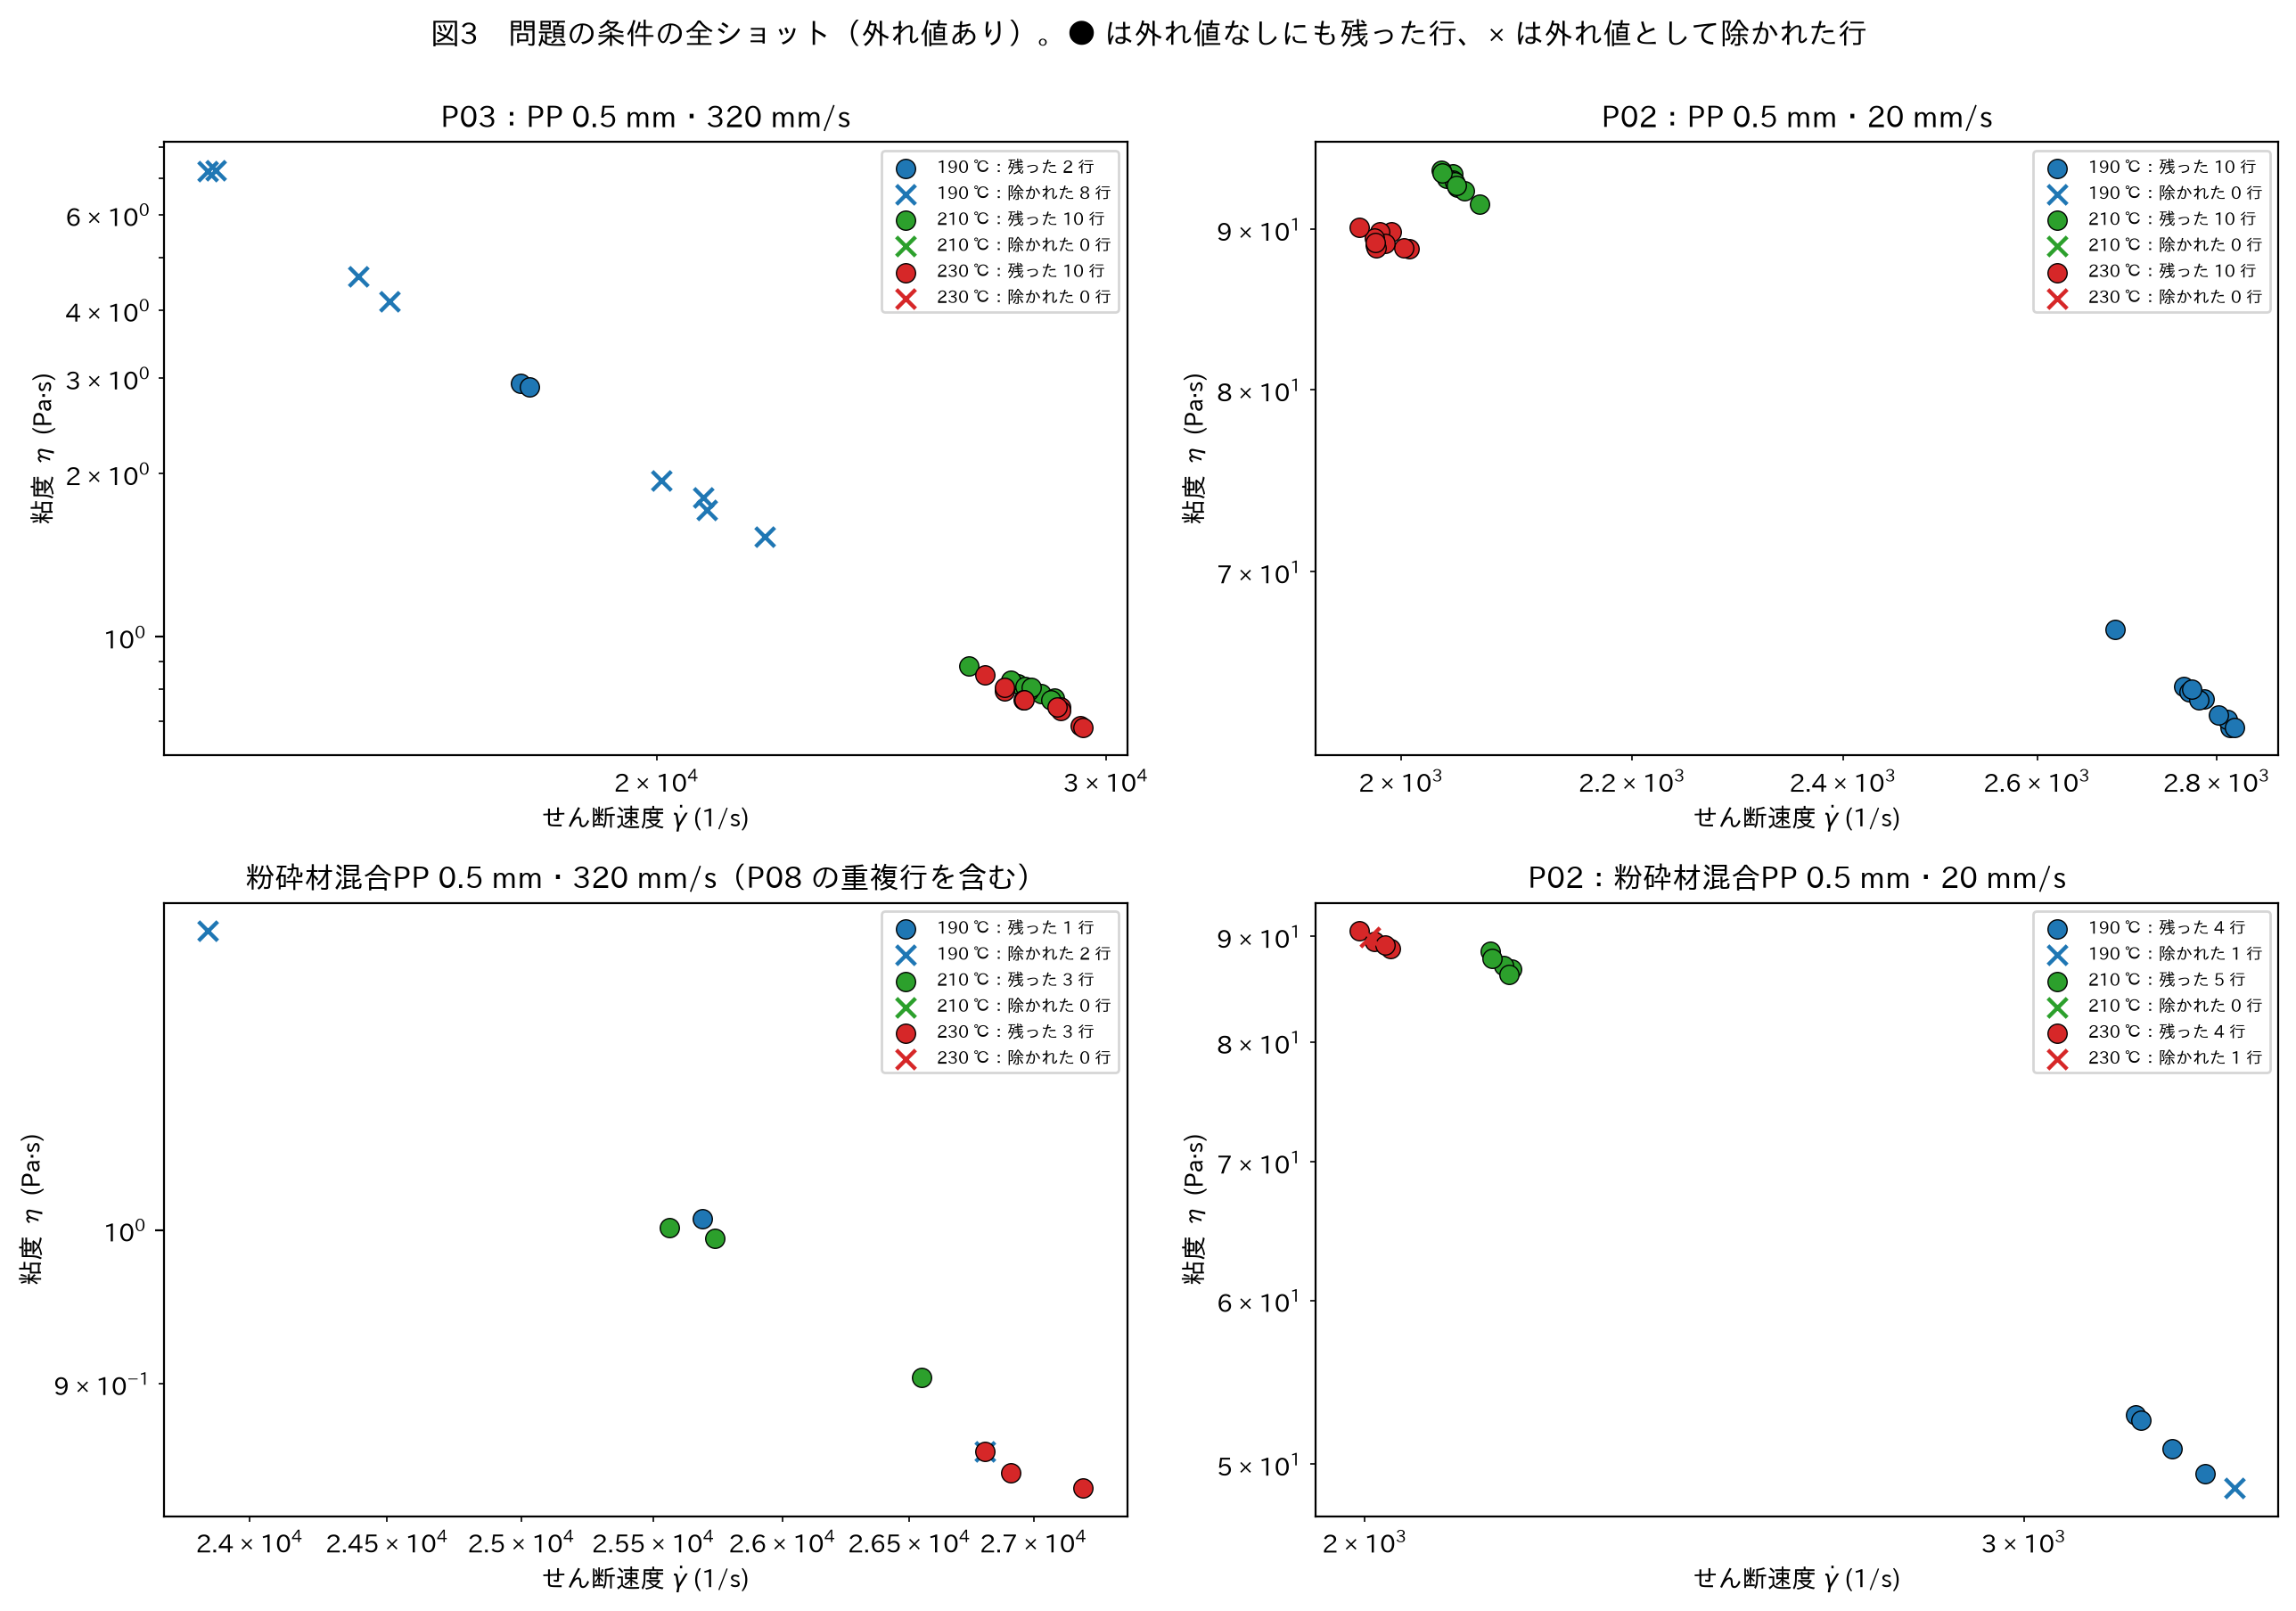
\includegraphics[width=0.95\linewidth]{fig3_problem_conditions.png}
\caption{問題の条件の、外れ値ありの全ショット。● は外れ値なしにも残った行、$\times$ は外れ値として除かれた行}
\end{figure}
\begin{points}
\pt{ファイル}\file{results/step3d/fig3_problem_conditions.png}
\pt{何を示す図か}一覧に載っている、問題の条件（P03、P02、粉砕材混合 PP の 190 ℃・0.5 mm・320 mm/s）を、外れ値ありのファイルの全ショットで見る図です。
\pt{軸と記号}横軸はせん断速度、縦軸は粘度（どちらも対数軸）。色は設定温度（青 190 ℃、緑 210 ℃、赤 230 ℃）。● は、外れ値なしのファイルにも残ったショット、$\times$ は、外れ値として除かれたショット。凡例に、行数を書いています。
\pt{見るポイント}190 ℃（青）の点が、210・230 ℃ の近くにあるか、離れているか。残った点（●）が、全ショットの代表になっているか。
\pt{今回の結果}P03（左上）は、10 ショットの粘度とせん断速度が、大きくばらつきます（せん断速度 14,000〜23,000 1/s、粘度 1.5〜7 Pa$\cdot$s と 4 倍以上）。そのうち 8 ショットが外れ値として除かれ、残った 2 ショット（● ）の平均は、ほかの条件から予測した値より約 23\% 高くなっています。同じ 0.5 mm・320 mm/s の 210・230 ℃ は、せん断速度約 28,000 1/s、粘度約 0.8 Pa$\cdot$s の近くに、ばらつきなく並んでいます。右上（P02）は、190 ℃ だけ、せん断速度が高く、粘度が低い条件で、10 ショットともそろっているので、外れ値ではなく、この条件の特徴として残しています（感度確認）。左下の粉砕材混合 PP は、190 ℃ の 3 ショットのうち、× が 2 行（1 行は 230 ℃ と同じ値の重複行 P08、1 行は外れ値判定）です。
\end{points}

% ---------------------------------------------------------------------
\subsection{図4：2 つの版の、分け方ごとの RMSE・NLPD（\file{fig4\_version\_metrics.png}）}
\begin{figure}[H]
\centering
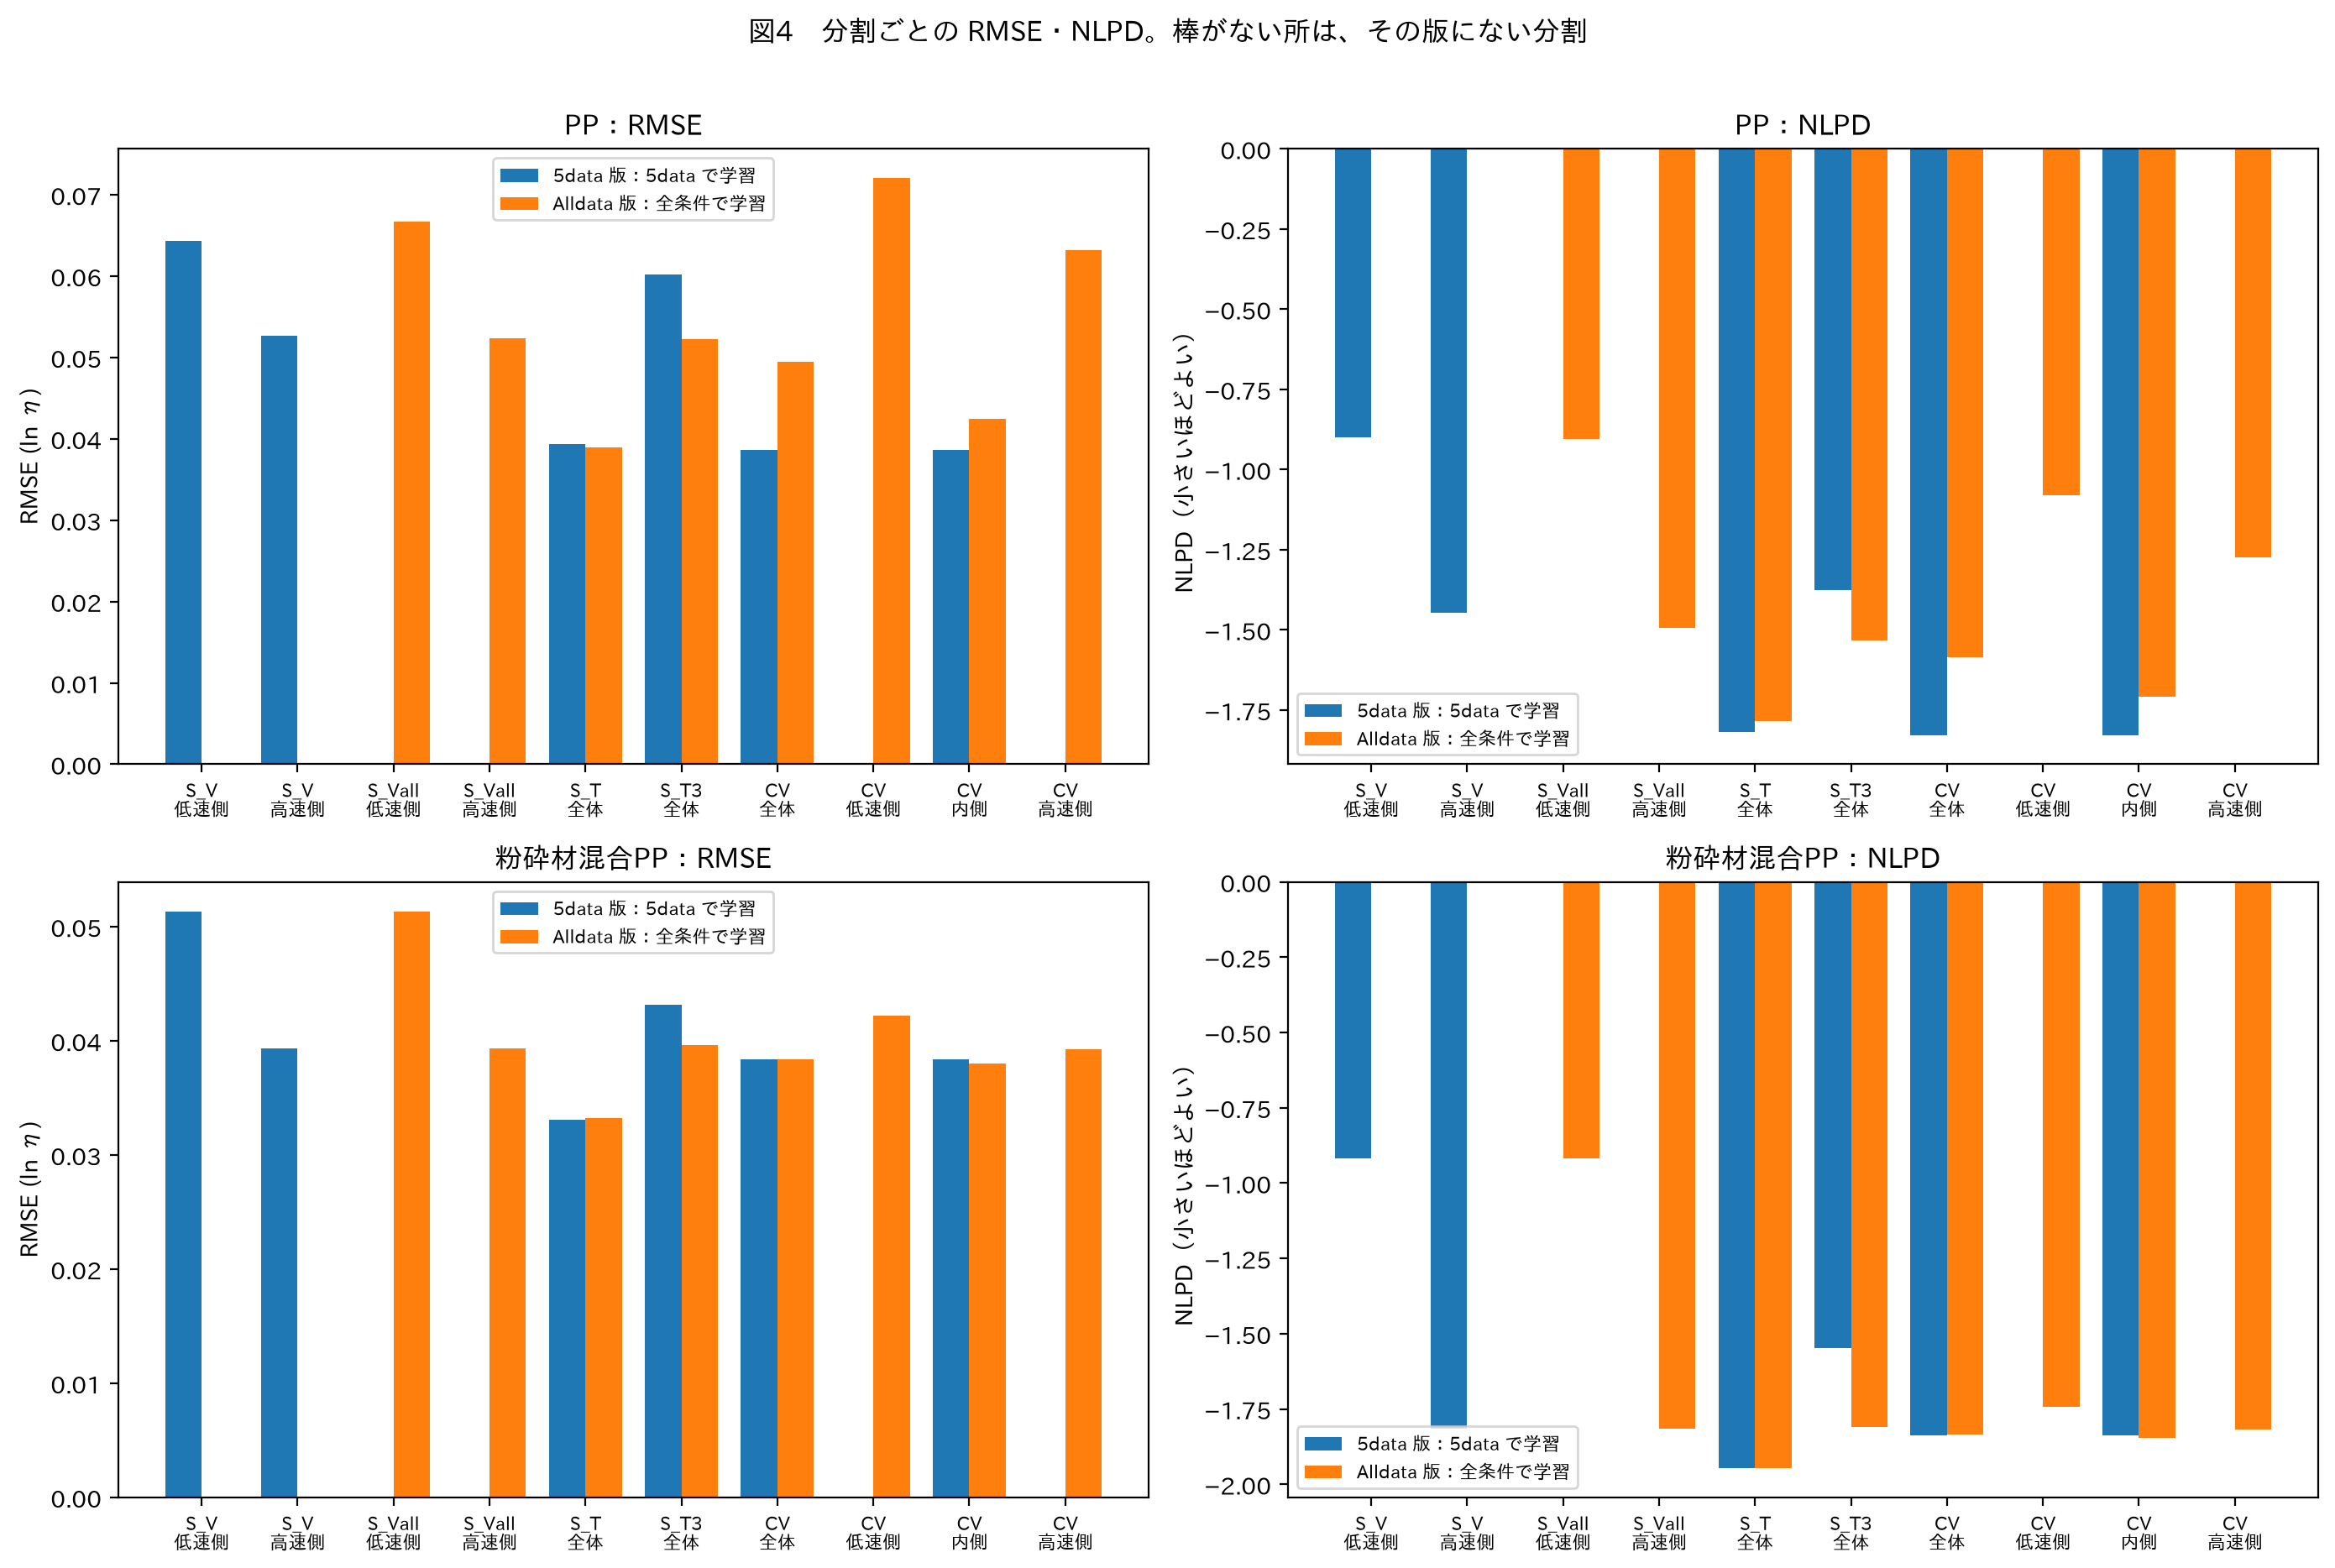
\includegraphics[width=0.95\linewidth]{fig4_version_metrics.png}
\caption{R3 の RMSE（左）と NLPD（右）。青：5data 版、橙：Alldata 版}
\end{figure}
\begin{points}
\pt{ファイル}\file{results/step3d/fig4_version_metrics.png}
\pt{何を示す図か}R3 で、2 つの版の精度を、分け方ごとに並べた図です。上が PP、下が粉砕材混合 PP。
\pt{軸と記号}横軸は、分け方と範囲（S\_V の低速側・高速側、S\_Vall、S\_T、S\_T3、CV の全体・低速側・内側・高速側）。縦軸は、RMSE（$\ln\eta$。小さいほど良い）と NLPD（小さいほど良い）。青が 5data 版、橙が Alldata 版。棒がない所は、その版にない分け方。
\pt{見るポイント}同じ分け方の青と橙が、同じ高さか。5data 版の S\_V と、Alldata 版の S\_Vall（どちらも 3data の外挿）が、近い値か。
\pt{今回の結果}外挿の検証（S\_V・S\_Vall）の RMSE は、PP の低速側が 0.064（5data 版）と 0.067（Alldata の 5data の条件）、高速側が 0.053 と 0.052 で、ほぼ同じです。S\_T（210 ℃）は、PP で 0.039 と 0.039、粉砕材混合 PP で 0.033 と 0.033 で、同等。S\_T3（3data の 210 ℃。外挿も重なる）は、Alldata 版のほうが小さく（PP 0.060 $\to$ 0.052、粉砕材混合 PP 0.043 $\to$ 0.040）、学習に、3data の条件（190・230 ℃）が入るためです。CV は、5data 版が 0.039（PP）、Alldata 版が 0.049 で、Alldata 版のほうが大きく出るのは、低速側・高速側の条件が含まれるためです（Alldata 版の低速側 0.072、高速側 0.063、内側 0.042）。
\end{points}

% ---------------------------------------------------------------------
\subsection{図5：予測と実測（\file{fig5\_parity.png}）}
\begin{figure}[H]
\centering
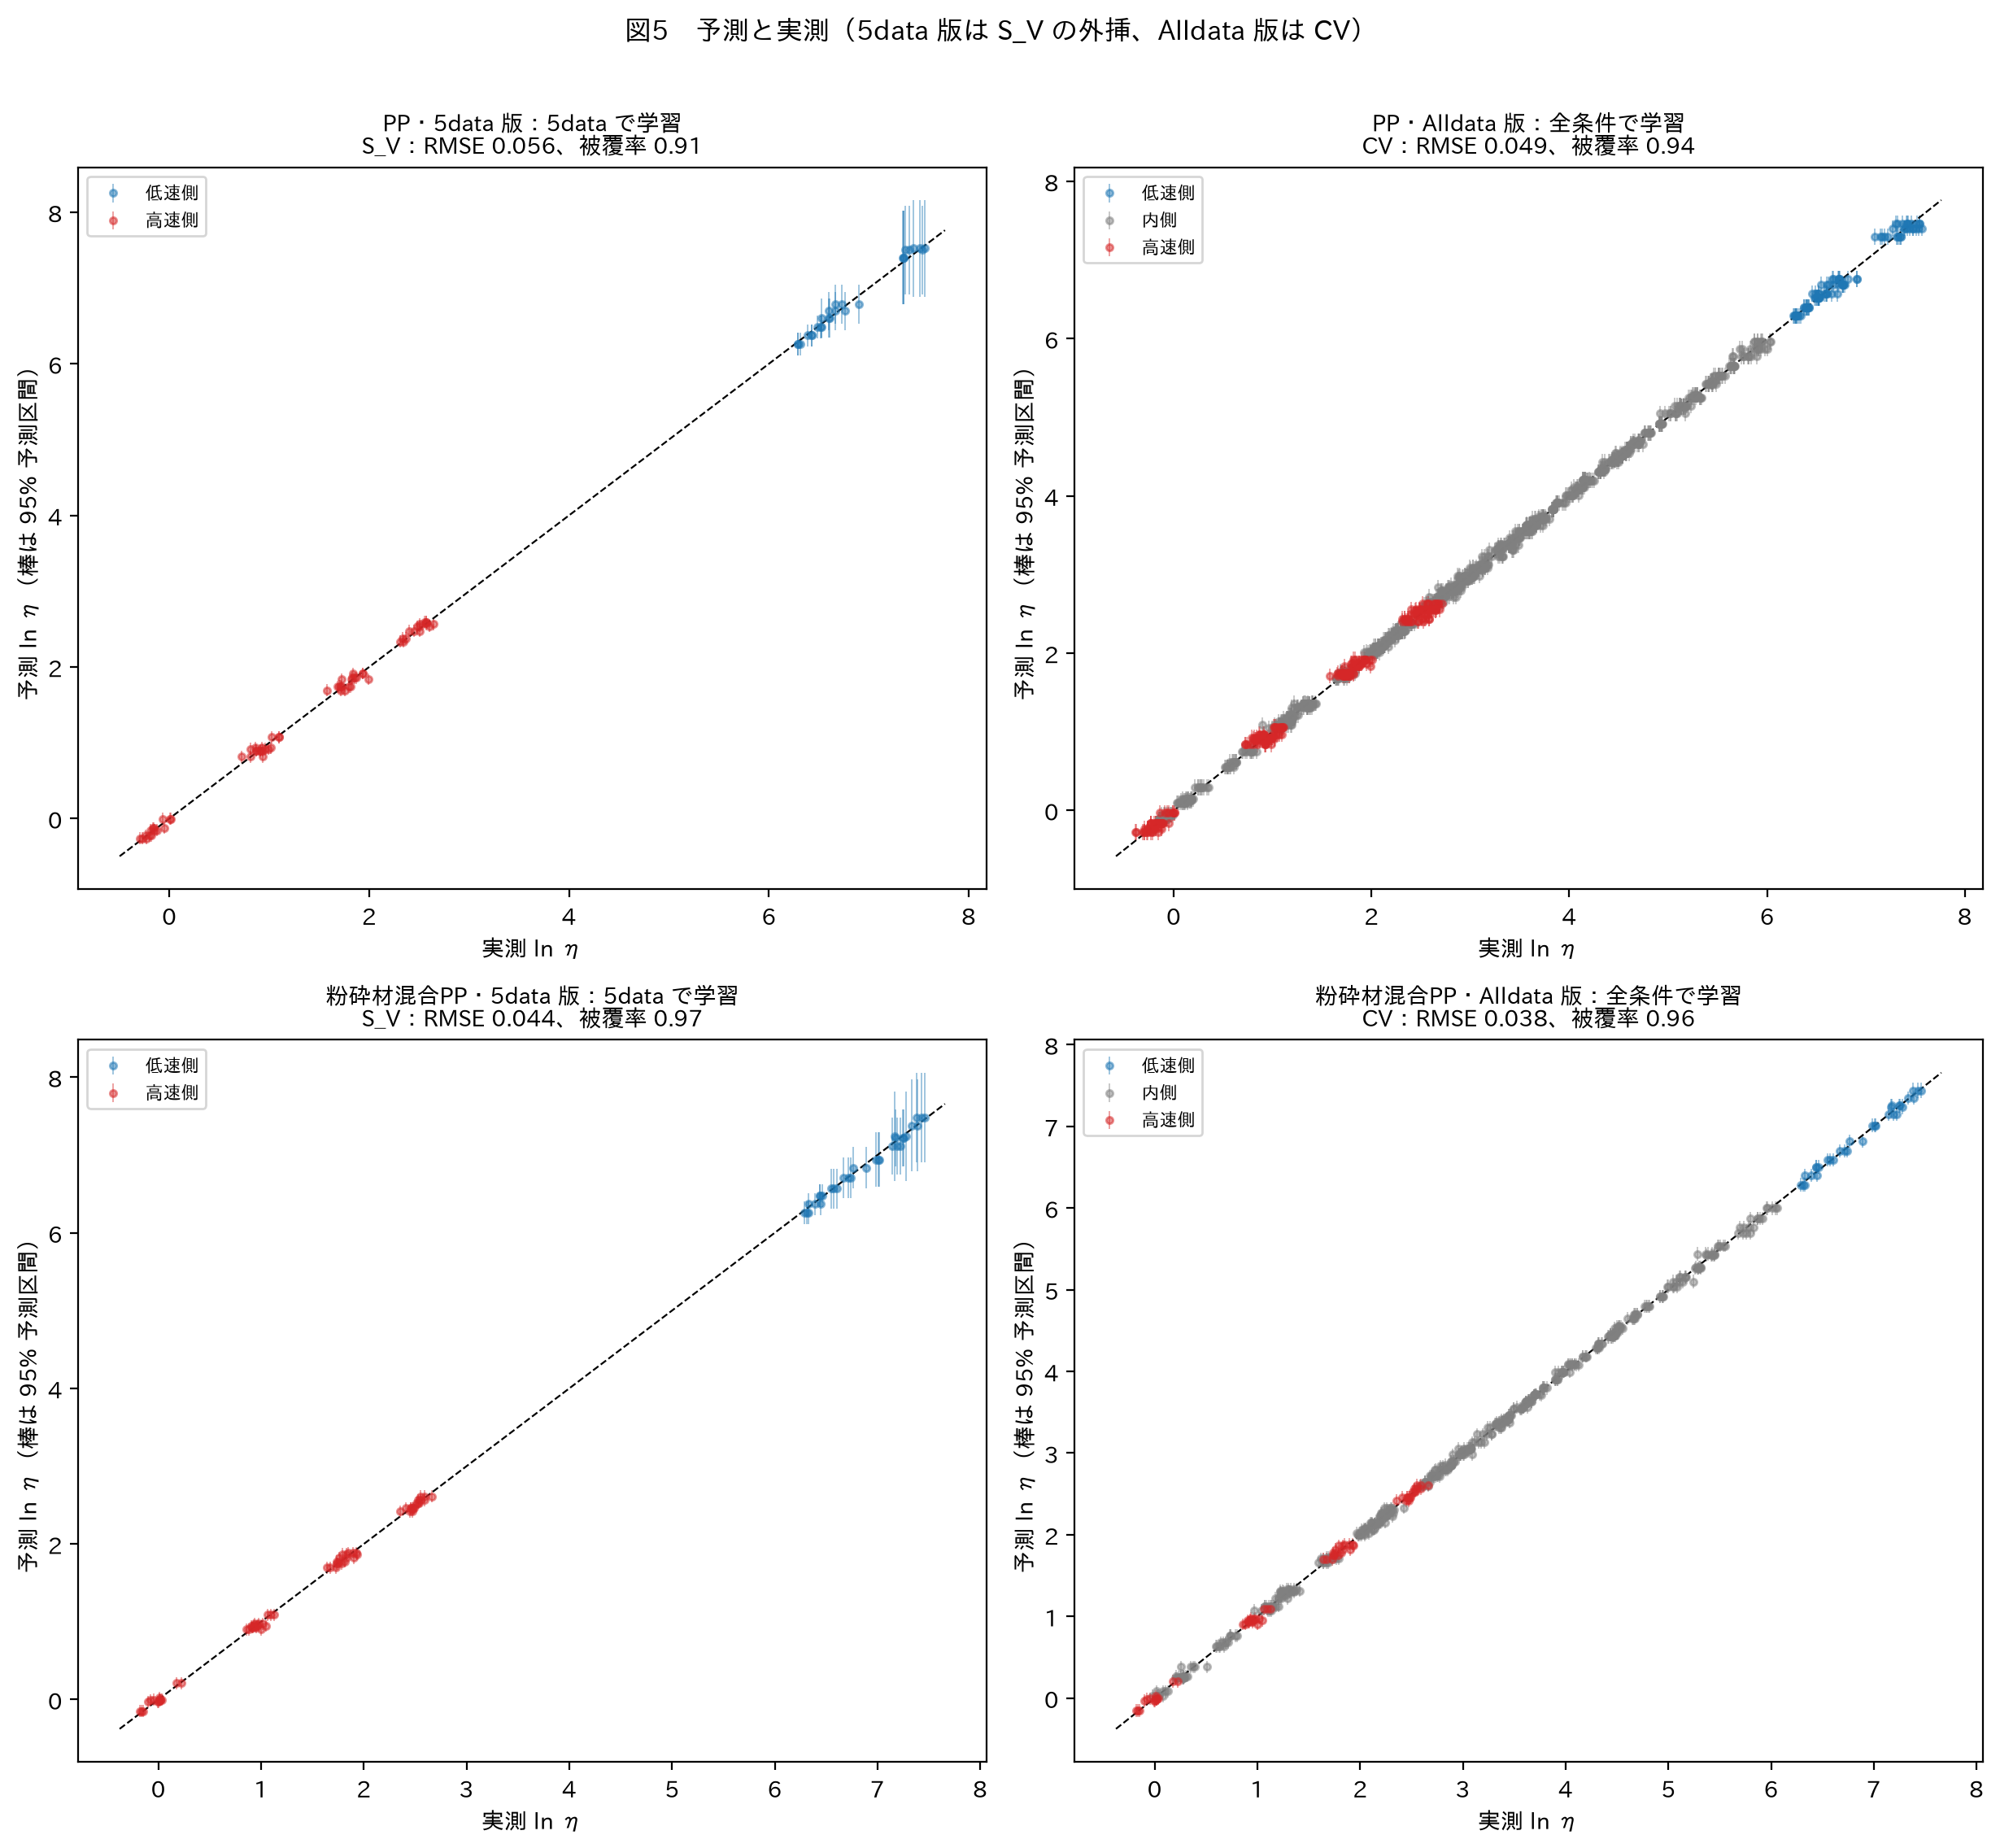
\includegraphics[width=0.85\linewidth]{fig5_parity.png}
\caption{予測と実測の $\ln\eta$。左が 5data 版の S\_V（外挿）、右が Alldata 版の CV。棒は 95\% 予測区間}
\end{figure}
\begin{points}
\pt{ファイル}\file{results/step3d/fig5_parity.png}
\pt{何を示す図か}予測が実測にどれだけ合うか（パリティ図）を見る図です。
\pt{軸と記号}横軸が実測の $\ln\eta$、縦軸が予測の $\ln\eta$。破線が一致する線。点の色は、青：低速側、灰：内側、赤：高速側。縦の棒が、95\% 予測区間。左が 5data 版（S\_V、3data を予測）、右が Alldata 版（CV）。
\pt{見るポイント}点が、破線の近くに並ぶか。棒が、破線をまたいでいるか（実測が区間に入っているか）。
\pt{今回の結果}点は、対角線（破線）の近くに並んでいます。5data 版の外挿（S\_V）では、低速側（青）の棒が長く（予測が不確か）、実測もその範囲に入ります（被覆率 PP 0.91、粉砕材混合 PP 0.97）。Alldata 版の CV は、棒が短く（予測が確か）、被覆率は PP 0.94、粉砕材混合 PP 0.96 です。
\end{points}

% ---------------------------------------------------------------------
\subsection{高解像度のグラフ（報告書・発表資料用）}
\begin{points}
\pt{ファイル}\file{results/step3d/highres/hr_<材料>_R3_<版>_by-thickness_<厚み>mm.png}（厚みごと）と、\file{..._by-temperature_<温度>C.png}（設定温度ごと）。Git には入れません（ノートのセルで、いつでも作り直せます）。
\pt{何を示す図か}GPR6月のノートのセル9-2 と同じ見せ方の、せん断速度 ― 粘度の学習結果グラフを、\textbf{600 dpi（15 $\times$ 10 インチ）}で 1 枚ずつ保存します。線は予測の平均、帯は 95\% 予測区間、塗りつぶしの点は学習の条件、白抜きの点は学習に使わなかった条件（5data 版の 3data）、黒い $\times$ は「感度確認」の条件（P02）です。版ごと（5data 版、Alldata 版）に描きます。
\pt{変え方}ノート8章の「高解像度のグラフ」のセルの先頭に、設定エリアがあります（描く版・材料、レイアウト、帯、点、軸の範囲、図の大きさ・解像度、文字の大きさ、保存形式など）。\textbf{そのセルの設定だけを直して、そのセルだけを実行し直せます}（学習はやり直しません。ノート全体を一度実行した後で）。
\pt{すべての図の高解像度版}手順3d 以降は、すべての図（図1〜図5）を、設定 \file{HR\_ALL} が True のとき、同じ名前で \file{highres/} にも 600 dpi で保存します。
\end{points}

% =====================================================================
\section{表の見方}

\begin{table}[H]
\caption{版の中身（\file{versions.csv}）。学習の行数・条件数と、検証データ。検証の行は、1 つの学習で、複数のテストを評価する場合を「，」で並べた}\label{tab:versions}
\begin{tabularx}{\linewidth}{@{}l>{\raggedright\arraybackslash}p{4\zw}>{\raggedright\arraybackslash}p{9\zw}rrX@{}}
\toprule
材料 & 版 & 分け方 & 学習の行数 & 条件数 & 検証 \\
\midrule
PP & 5data & ALL（最終モデル） & 460 & 93 & --- \\
 &  & S\_V & 460 & 93 & 3data：93 行 32 条件 \\
 &  & S\_T & 307 & 62 & 5data の 210 ℃：153 行 31 条件，3data の 210 ℃：31 行 11 条件 \\
 &  & CV（10 分割。1 分割の例） & 410 & 83 & テスト：50 行 10 条件 \\
 & Alldata & ALL（最終モデル） & 1234 & 125 & --- \\
 &  & S\_T & 819 & 83 & 5data の 210 ℃：153 行 31 条件，3data の 210 ℃：31 行 11 条件 \\
 &  & S\_Vall & 921 & 93 & 3data：93 行 32 条件 \\
 &  & CV（10 分割。1 分割の例） & 1106 & 112 & テスト：128 行 13 条件 \\
粉砕材混合 PP & 5data & ALL（最終モデル） & 459 & 93 & --- \\
 &  & S\_V & 459 & 93 & 3data：101 行 36 条件 \\
 &  & S\_T & 305 & 62 & 5data の 210 ℃：154 行 31 条件，3data の 210 ℃：35 行 12 条件 \\
 &  & CV（10 分割。1 分割の例） & 410 & 83 & テスト：49 行 10 条件 \\
 & Alldata & ALL（最終モデル） & 560 & 129 & --- \\
 &  & S\_T & 371 & 86 & 5data の 210 ℃：154 行 31 条件，3data の 210 ℃：35 行 12 条件 \\
 &  & S\_Vall & 459 & 93 & 3data：101 行 36 条件 \\
 &  & CV（10 分割。1 分割の例） & 497 & 116 & テスト：63 行 13 条件 \\
\bottomrule
\end{tabularx}
\end{table}

\begin{table}[H]
\caption{ファイルの包含関係（\file{inclusion.csv}）。「Alldata にある」：5data・3data の行のうち、Alldata に同じ行（元ファイル名と、$\eta$・$\gd$・\PI・\PII・$\Tff$ が一致）がある数。最後の行は、逆（Alldata の行のうち、5data・3data のどちらにもある／ない）}\label{tab:incl}
\begin{tabularx}{\linewidth}{@{}l>{\raggedright\arraybackslash}p{3\zw}>{\raggedright\arraybackslash}p{13\zw}rrr@{}}
\toprule
材料 & 外れ値 & 組 & 行数 & ある & ない \\
\midrule
PP & あり & 5data & 465 & 465 & 0 \\
 &  & 3data & 96 & 96 & 0 \\
 &  & Alldata（5data・3data との逆） & 1250 & 561 & 689 \\
 & なし & 5data & 460 & 456 & 4 \\
 &  & 3data & 93 & 93 & 0 \\
 &  & Alldata（5data・3data との逆） & 1234 & 549 & 685 \\
粉砕材混合 PP & あり & 5data & 465 & 465 & 0 \\
 &  & 3data & 107 & 107 & 0 \\
 &  & Alldata（5data・3data との逆） & 572 & 572 & 0 \\
 & なし & 5data & 459 & 459 & 0 \\
 &  & 3data & 101 & 101 & 0 \\
 &  & Alldata（5data・3data との逆） & 560 & 560 & 0 \\
\bottomrule
\end{tabularx}
\end{table}

\begin{table}[H]
\caption{ショットの順番によるずれ（Alldata。\file{shot\_drift.csv}）。傾き：1 ショットあたり（括弧は標準誤差）。ずれ：最初 $\to$ 最後（傾き $\times$ 順番の幅）。後半 $-$ 前半：順番 6 以降の平均 $-$ 順番 5 以前の平均（PP のみ。括弧は標準誤差）}\label{tab:drift}
\begin{tabularx}{\linewidth}{@{}l>{\raggedright\arraybackslash}p{3\zw}lr>{\raggedright\arraybackslash}p{9\zw}rX@{}}
\toprule
材料 & 外れ値 & 量 & 条件数 & 傾き（標準誤差） & ずれ & 後半 $-$ 前半 \\
\midrule
PP & なし & $\ln\eta$ & 125 & $-0.00109$（0.00051） & $-0.0098$ & $-0.0049$（0.0025） \\
 &  & $\ln\gd$ & 125 & 0.00039（0.00023） & 0.0035 & 0.0017（0.0012） \\
 & あり & $\ln\eta$ & 125 & $-0.00033$（0.00059） & $-0.0029$ & $-0.0007$（0.0028） \\
 &  & $\ln\gd$ & 125 & 0.00008（0.00026） & 0.0008 & 0.0000（0.0012） \\
粉砕材混合 PP & なし & $\ln\eta$ & 123 & $-0.00014$（0.00129） & $-0.0006$ & --- \\
 &  & $\ln\gd$ & 123 & 0.00009（0.00055） & 0.0004 & --- \\
 & あり & $\ln\eta$ & 128 & $-0.00071$（0.00159） & $-0.0028$ & --- \\
 &  & $\ln\gd$ & 128 & 0.00071（0.00105） & 0.0029 & --- \\
\bottomrule
\end{tabularx}
\end{table}

\begin{table}[H]
\caption{規則 f の結果（\file{outlier\_check.csv}）。全条件：除外する前。除外後：一覧の「除外」を除いた後。$z$ と残差は、$|z|$ が最大の条件のもの}\label{tab:outlier}
\begin{tabularx}{\linewidth}{@{}l>{\raggedright\arraybackslash}p{3\zw}rrrX r@{}}
\toprule
材料 & データ & 条件数 & 拾った数 & $z$ & 条件 & 残差 \\
\midrule
PP & 全条件 & 129 & 1（P03） & 9.2 & 190\_0.5\_320 & 0.206 \\
 & 除外後 & 125 & 0 & 3.9 & 210\_2.0\_3 & 0.034 \\
粉砕材混合 PP & 全条件 & 129 & 0 & 4.0 & 190\_1.5\_10 & 0.057 \\
 & 除外後 & 129 & 0 & 4.0 & 190\_1.5\_10 & 0.057 \\
\bottomrule
\end{tabularx}
\end{table}

\begin{table}[H]
\caption{R3 の RMSE（$\ln\eta$。\file{metrics.csv}）。小さいほど良い。S\_V は 5data 版、S\_Vall は Alldata 版の外挿}\label{tab:rmse}
\begin{tabularx}{\linewidth}{@{}l>{\raggedright\arraybackslash}p{3.5\zw}*{7}{r}@{}}
\toprule
 & & \multicolumn{2}{c}{外挿：低速側} & \multicolumn{2}{c}{外挿：高速側} & S\_T & S\_T3 & CV \\
\cmidrule(lr){3-4}\cmidrule(lr){5-6}
材料 & 版 & S\_V & S\_Vall & S\_V & S\_Vall & 全体 & 全体 & 全体 \\
\midrule
PP & 5data & 0.064 & --- & 0.053 & --- & 0.039 & 0.060 & 0.039 \\
 & Alldata & --- & 0.067 & --- & 0.052 & 0.039 & 0.052 & 0.049 \\
粉砕材混合 PP & 5data & 0.051 & --- & 0.039 & --- & 0.033 & 0.043 & 0.038 \\
 & Alldata & --- & 0.051 & --- & 0.039 & 0.033 & 0.040 & 0.038 \\
\bottomrule
\end{tabularx}
\end{table}

\begin{table}[H]
\caption{R3 の 95\% 予測区間の被覆率（0.95 に近いほど、区間の広さが適切）}\label{tab:cov}
\begin{tabularx}{\linewidth}{@{}l>{\raggedright\arraybackslash}p{3.5\zw}*{7}{r}@{}}
\toprule
 & & \multicolumn{2}{c}{外挿：低速側} & \multicolumn{2}{c}{外挿：高速側} & S\_T & S\_T3 & CV \\
\cmidrule(lr){3-4}\cmidrule(lr){5-6}
材料 & 版 & S\_V & S\_Vall & S\_V & S\_Vall & 全体 & 全体 & 全体 \\
\midrule
PP & 5data & 1.00 & --- & 0.88 & --- & 0.93 & 0.94 & 0.95 \\
 & Alldata & --- & 1.00 & --- & 0.91 & 0.97 & 0.90 & 0.94 \\
粉砕材混合 PP & 5data & 1.00 & --- & 0.96 & --- & 0.97 & 0.97 & 0.95 \\
 & Alldata & --- & 1.00 & --- & 0.96 & 0.97 & 0.97 & 0.96 \\
\bottomrule
\end{tabularx}
\end{table}

\begin{table}[H]
\caption{R3 の NLPD（小さいほど良い）}\label{tab:nlpd}
\begin{tabularx}{\linewidth}{@{}l>{\raggedright\arraybackslash}p{3.5\zw}*{7}{r}@{}}
\toprule
 & & \multicolumn{2}{c}{外挿：低速側} & \multicolumn{2}{c}{外挿：高速側} & S\_T & S\_T3 & CV \\
\cmidrule(lr){3-4}\cmidrule(lr){5-6}
材料 & 版 & S\_V & S\_Vall & S\_V & S\_Vall & 全体 & 全体 & 全体 \\
\midrule
PP & 5data & $-0.90$ & --- & $-1.45$ & --- & $-1.82$ & $-1.38$ & $-1.83$ \\
 & Alldata & --- & $-0.90$ & --- & $-1.49$ & $-1.79$ & $-1.53$ & $-1.58$ \\
粉砕材混合 PP & 5data & $-0.92$ & --- & $-1.82$ & --- & $-1.95$ & $-1.55$ & $-1.84$ \\
 & Alldata & --- & $-0.92$ & --- & $-1.82$ & $-1.95$ & $-1.81$ & $-1.84$ \\
\bottomrule
\end{tabularx}
\end{table}

\begin{table}[H]
\caption{最終モデルのノイズ（\file{kernels.csv}）。ノイズ：GPR のノイズの標準偏差。純粋誤差：同じ条件内の $\ln\eta$ の標準偏差。LML：対数周辺尤度}\label{tab:kern}
\begin{tabularx}{\linewidth}{@{}l>{\raggedright\arraybackslash}p{3.5\zw}rrrrrr@{}}
\toprule
材料 & 版 & 学習の行数 & 条件数 & ノイズ & 純粋誤差 & 比 & LML \\
\midrule
PP & 5data & 460 & 93 & 0.0385 & 0.0409 & 0.94 & 775.3 \\
 & Alldata & 1234 & 125 & 0.0493 & 0.0508 & 0.97 & 1880.6 \\
粉砕材混合 PP & 5data & 459 & 93 & 0.0374 & 0.0393 & 0.95 & 785.7 \\
 & Alldata & 560 & 129 & 0.0377 & 0.0403 & 0.94 & 959.9 \\
\bottomrule
\end{tabularx}
\end{table}

\begin{table}[H]
\caption{\file{results/step3d/} の表}
\begin{tabularx}{\linewidth}{@{}>{\raggedright\arraybackslash}p{19\zw}X@{}}
\toprule
ファイル & 中身と主な列 \\
\midrule
\file{versions.csv} & 版ごとの、学習・検証の行数と条件数。\file{n_train}、\file{n_cond_train}、\file{shots_per_cond}、\file{gd_range}、\file{tests}、\file{removed_by_list}（問題データ一覧の「除外」で除いた行数）。 \\
\file{inclusion.csv} & 包含関係。\file{n_rows}、\file{n_in_alldata}、\file{n_not_in_alldata}。 \\
\file{shot_drift.csv} & ショットの順番によるずれ。\file{slope_per_shot}、\file{se}、\file{drift_first_to_last}、\file{z}、\file{half_diff}。群（全体・設定温度・厚み・射出速度）ごとと、4 つの量（$\ln\eta$、$\ln\gd$、$\ln$\PI、$\Tff$）。 \\
\file{outlier_check.csv} & 規則 f の結果。条件ごとの \file{resid}、\file{sd}、\file{z}、\file{flag}、\file{list_id}（問題データ一覧の ID）、\file{data}（全条件／除外後）。 \\
\file{problem_conditions.csv} & 図3 の、問題の条件の集計（残ったショット数など）。 \\
\file{metrics.csv} & 版・分け方・範囲ごとの指標（\file{RMSE}、\file{R2}、\file{coverage95}、\file{NLPD}、\file{mean_sd}、\file{noise_sd}）。 \\
\file{kernels.csv} & 学習した GPR のハイパーパラメータ（\file{amplitude}、\file{ls_*}、\file{noise_sd}、\file{LML} など）と、純粋誤差、学習にかかった秒数。 \\
\file{summary.csv} & 版ごとのまとめ（行数・条件数・主な RMSE・ノイズ）。 \\
\bottomrule
\end{tabularx}
\end{table}

% =====================================================================
\section{結果のまとめ}

\subsection{観点ごとの結論}
\begin{enumerate}[itemsep=0.6ex,topsep=0.6ex]
\item \textbf{今後使う学習データは、外れ値なしの 2 つの版}：5data 版（5data で学習、3data で外挿を検証）と、Alldata 版（全条件で学習）です。どちらも、問題データ一覧の「除外」（P01・P03・P08）を除きます。外れ値ありは、今後は使いません。ノートの設定 \texttt{DATA\_VERSIONS} で、どちらでも、両方でも検討できます。
\item \textbf{ファイルの包含関係は、予想どおり}：外れ値ありでは、5data・3data の全行が Alldata にあり、粉砕材混合 PP は 5data と 3data を合わせたものが Alldata と一致します（表\ref{tab:incl}）。外れ値なしでは、外れ値の除き方がファイルごとに違うため、PP の 5data の 4 行が Alldata にありません。
\item \textbf{Alldata の後半のショットを足しても、粘度はずれない}：ショットの順番によるずれは、PP で $-0.0098$（9 ショット分。粘度の約 1.0\%）と、許容値の 0.02 よりずっと小さく、粉砕材混合 PP も同様です（図1、表\ref{tab:drift}）。群ごとに見ると、最大は PP の 射出速度 低速側（3・5 mm/s） の $-0.0416$（粘度で約 4\%）で、許容値の 2 倍（0.04）をわずかに超えますが、傾きは標準誤差の約 1.8 倍で、偶然の範囲です（9 条件しかなく、標準誤差が大きいため。「順番 6 以降 $-$ 5 以前」は $-0.0207$）。Alldata 版の学習データとして使えます。
\item \textbf{外れ値は、P03 だけ（除外に変更）}：規則 f で拾ったのは、PP の 190 ℃・0.5 mm・320 mm/s（P03）だけでした（z = 9.2）。ユーザーの指示（「検知したら、一覧に記録して、除いてよい」）に従い、P03 を「感度確認」から「除外」に変えました。除いた後に、新しく拾われる条件は 0 件です（図2、表\ref{tab:outlier}）。
\item \textbf{2 つの版は、同じモデル（R3）で、同等の精度}：S\_T は、PP で 0.039（5data 版）と 0.039（Alldata 版）、粉砕材混合 PP で 0.033 と 0.033。Alldata 版の外挿（S\_Vall）も、5data 版（S\_V）と同じ水準です。ショットが増えても、悪くなりません（図4、表\ref{tab:rmse}）。
\item \textbf{Alldata 版の利点は、両端の条件も学習に入ること}：Alldata 版の最終モデルは、低速側・高速側の条件も学習しているので、予測の区間が狭く（ノイズの標準偏差 PP 0.049、純粋誤差 0.051）、両端の外側でない限り、外挿に頼りません。この利点は、同じデータの中の検証（CV）では測れません。5data 版の外挿の成績が、両端を学習に入れない場合の目安です。
\item \textbf{使い分け}：5data 版は、「学習の外側をどれだけ当てられるか」を確かめるときの版（モデルの性能評価）、Alldata 版は、最終的な予測モデル（全条件を使う）の版、という使い分けを想定しています。手順5 の本実装（構造 B・A）は、この 2 つの版に当てはめて、比べます。
\end{enumerate}

\subsection{ノートの「★要確認」の意味}
ノートの \texttt{★要確認} は、想定と違う、または注意が要る点です。この文書の時点で出る主なものと、その意味は次のとおりです。
\begin{points}
\pt{5data 版の S\_V 低速側の被覆率が 1.00}95\% 区間に、低速側の検証データがすべて入っています（PP・粉砕材混合 PP とも）。区間が広め（保守的）という意味で、外れるより安全です。低速側は、学習していない範囲の外挿なので、広めに出ること自体は正しい振る舞いです（手順3b の R3 と同じ）。
\pt{PP・5data 版の S\_V 高速側の被覆率 0.88}0.90 を少し下回ります。高速側の予測の幅が狭く（予測標準偏差の平均 0.041）、外れる条件（66 行中 8 行）があるためです（P03 は、すでに除外した後の値です）。Alldata の 5data の条件で学習した S\_Vall では 0.91、ショットの増えた Alldata 版の S\_T3 では 0.90 です。
\pt{ショットの順番によるずれ（群ごと）}最大は PP の 射出速度 低速側（3・5 mm/s） の $-0.0416$（粘度で約 4\%）で、許容値の 2 倍（0.04）をわずかに超えますが、傾きは標準誤差の約 1.8 倍で、偶然の範囲です（9 条件しかなく、標準誤差が大きいため。「順番 6 以降 $-$ 5 以前」は $-0.0207$）。
\pt{Alldata 版の CV で、低速側・高速側の被覆率が低め}PP の CV の低速側は 0.84、高速側は 0.85 で、内側（0.97）より低めです。両端の条件は、その外側に学習データがなく、予測が外挿になるためです（ノートの判定は、CV 全体の被覆率で行っています）。
\end{points}

\subsection{次の手順と、ユーザーに決めてほしいこと}
\begin{points}
\pt{P03 の「除外」への変更}規則 f で拾った PP の 190 ℃・0.5 mm・320 mm/s（P03）を、ユーザーの指示に従って「除外」に変えました。これは、10 月 12 日の「主の分析では残す」という決定を、改めたことになります。手順3a〜5a の結果は、P03 を残したときの記録で、作り直すと P03 が除かれます（3b・3c の説明書の P03 に関する文は、作り直すときに直す必要があります）。
\pt{手順5（本実装）}構造 B（本命）と A（対案）を、同じ形で実装し、この 2 つの版に当てはめて比べます（基準は、構造なしの通常の GPR、R3）。最終モデルに、MCMC を使うかも、そこで相談します。
\pt{手順6（ばらつきの分析）}Alldata 版は、1 条件のショットが多い（PP は 10 回）ので、同じ条件のばらつき（純粋誤差）の分析にも向いています。
\end{points}

\end{document}
